\section{Data Preprocessing}

Data preprocessing is the process of preparing raw data for analysis by cleaning and transforming it into a usable format. In data mining it refers to preparing raw data for mining by performing tasks like cleaning, transforming, and organizing it into a format suitable for mining algorithms.

Goal is to improve the quality of the data, handling missing values, removing duplicates, and normalizing data to ensures the accuracy and consistency of the dataset.

\subsection{Data Cleaning}

In this step, we focus on cleaning the dataset to prepare it for analysis.

\begin{enumerate}
\item \textbf{Check For Null Values:}

We should identify any missing values across the dataset, and decide how to handle them (impute, drop, or analyze separately). For this particular dataset no null values were found.

\begin{verbatim}
sum(is.na(df_climate))
\end{verbatim}

\item\textbf{Drop the unnecessary columns:}

In our data set the first column consisting of an index is not necessary so we can drop the first unnamed column from our climate dataset.

\begin{verbatim}
df_climate$X <- NULL
\end{verbatim}

\item\textbf{Inspect the Duplicate Columns:}

We must also check for duplicate columns and remove them as they don't provide any additional information. For this particular climate dataset no such columns were found.

\begin{verbatim}
duplicated(colnames(df_climate))
\end{verbatim}

\item\textbf{Convert Date Column to Date Format:}

Since the Date column is currently in character format, convert it to Date using \texttt{as.Date()}.

\begin{verbatim}
df_climate$Date <- as.Date(df_climate$Date, format = "%Y-%m-%d")
\end{verbatim}

\item \textbf{Set Date as Index:}

Setting the date as an index is not strictly necessary in R for time series data analysis, but it is often a good practice and can simplify time-based operations. Setting the date as an index (or primary column) helps in slicing, filtering, and aggregating data by time periods. For this data set I used \texttt{tsibble} package.

\begin{verbatim}
# Convert tibble to tsibble
df_climate <- as_tsibble(df_climate, index = Date, key = District)

# Check for index
index_name <- index_var(df_climate)
print(index_name)
\end{verbatim}

The dataset structure after cleaning looks like:

\begin{verbatim}
glimpse(df_climate)
\end{verbatim}

% Figure here ---------------------------
\begin{figure}[h!]
    \centering
    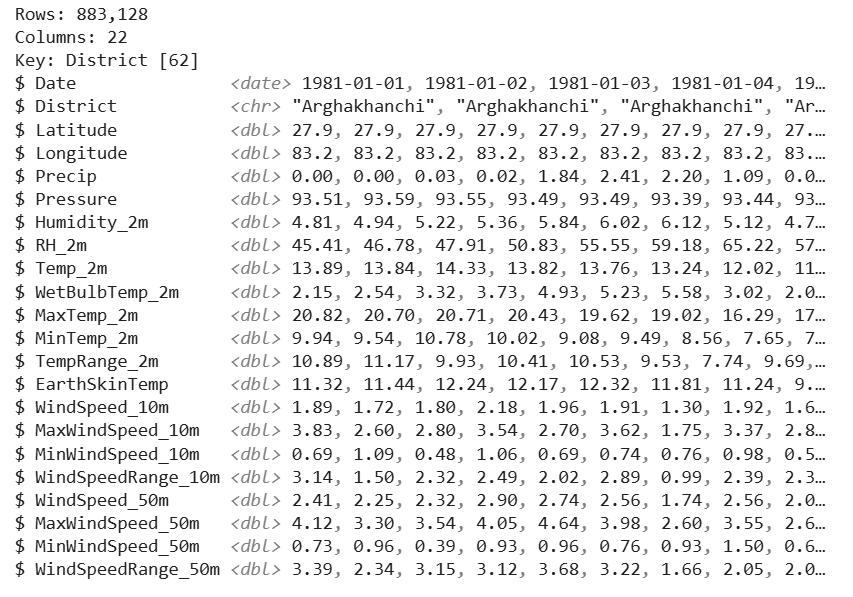
\includegraphics[width=0.6\textwidth]{figures/glimpse.png}
    \caption{Glimpse of the Cleaned Climate Dataset.}
\end{figure}

\end{enumerate}
\subsection{Feature Engineering}

Feature engineering is the process of taking raw data and transforming it into meaningful inputs that help a machine learning model understand patterns better. Think of it like preparing ingredients before cooking like when you chop, mix, and season them so the final dish tastes great.

In data analysis, this means creating new variables, cleaning data, selecting important information, or combining features to improve the model’s ability to make accurate predictions. Good feature engineering can often make a bigger difference in model performance than just using more complex algorithms.

It helps to create new features that might be helpful for your analysis. For this dataset, we can derive the month column from Date. Since Date is in format YYYY-MM-DD, we can extract the month and create a new column called month number. We can also create another column called month label and assign the names of the month (e.g., 1 = Jan, 2 = Feb, and so on).

\begin{verbatim}
# Extract month as number and label
df_climate$Month_Number <- month(df_climate$Date)     
df_climate$Month_Label <- month(df_climate$Date, label = TRUE)
\end{verbatim}

We can categorize the months into season and create a new column called “Season” for seasonal data analysis in the following way:

\begin{verbatim}
# Categorize months into seasons
df_climate <- df_climate %>%
  mutate(Season = case_when(
    month(Date) %in% c(12, 1, 2)  ~ "Winter",
    month(Date) %in% c(3, 4, 5)   ~ "Spring",
    month(Date) %in% c(6, 7, 8)   ~ "Summer",
    month(Date) %in% c(9, 10, 11) ~ "Fall"
  ))
\end{verbatim}

In R we can use \texttt{dplyr} and \texttt{lubridate} to extract the components of date. The function called \texttt{mutate()} can be used for creation of new columns and modifying the existing columns in our case.
